\chapter{Izvod matematičkog modela}

Za mehanizam sa slike \ref{fig:mehanizma} potrebno je izvršiti optimalnu sintezu dimenzija mehanizma tako da bi moment na ručici $A_0A$ bio konstantan. U cilindru se nalazi idealni plin i cijeli proces se odvija pri konstantnoj temperaturi. Zadane su slijedeće vrijednosti:
\begin{align*}
h_1&=250\ \text{mm}\\
h_2&=75\ \text{mm}\\
F_1&=18\ \text{N}\\
\Delta \varphi &=\frac{\pi}{3}\\
A&=konst
\end{align*}

\begin{figure}[H]
\center
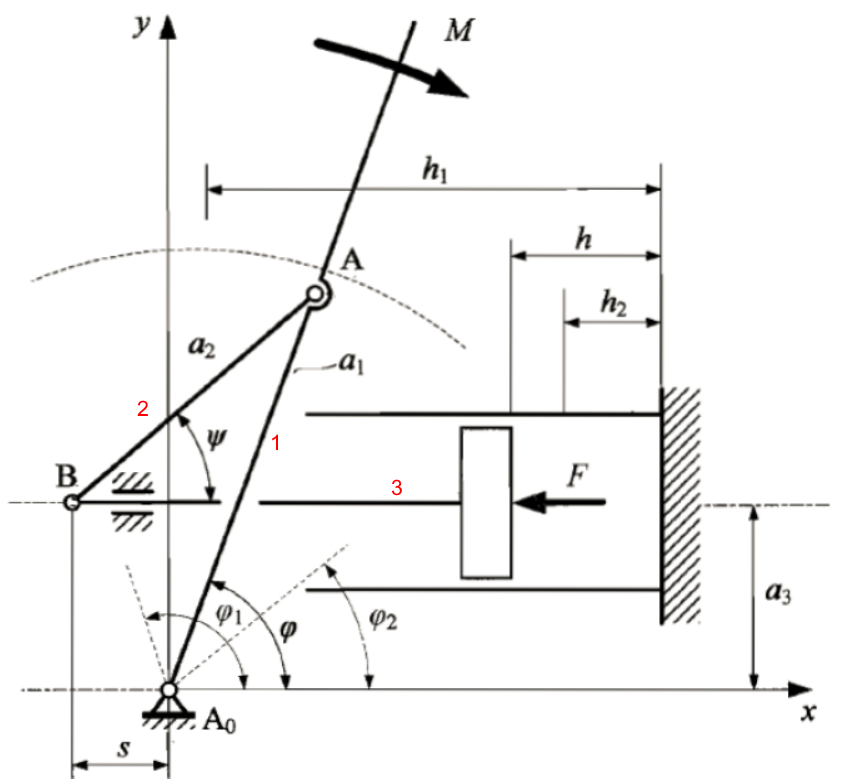
\includegraphics[scale=.4]{slike/mehanizam.png}
\caption[Skica mehanizma za optimiranje]{Skica mehanizma za optimiranje \cite{Chiang2000}}
\label{fig:mehanizma}
\end{figure}

\section{Izvod funkcije cilja}
\quad Za konstantu temperaturu i eksponent politrope $n=1$ dobivamo ravnotežnu promjenu stanja kod koje se temperatura radnog medija ne mijenja tj. $T_1=T_2=T$ i $\Delta T=0$.\\

Jednadžbe stanja:
\begin{equation}
\label{eq:stanje1}
p_1V_1=mRT_1
\end{equation}
\begin{center}
i
\end{center}
\begin{equation}
\label{eq:stanje2}
p_2V_2=mRT_2
\end{equation}

povezane uvjetom $T_1=T_2=T$ daju sljedeću jednadžbu stanja:
\begin{equation}
\label{eq:stanje}
p_1V_1=p_2V_2=pV
\end{equation}

Volumen u cilindru računa se prema formuli \ref{eq:volumen} dok se sila na klip računa po izrazu \ref{eq:sila}.
\begin{equation}
\label{eq:volumen}
V=Ah
\end{equation}
\begin{equation}
\label{eq:sila}
F=pA
\end{equation}

Uvrstimo li izraze \ref{eq:volumen} i \ref{eq:sila} u jednadžbu \ref{eq:stanje} dobije se slijedeća jednadžba:
\begin{gather}
\dfrac{F_1}{A}h_1A=\dfrac{F_2}{A}h_2A=\dfrac{F}{A}hA\\
\label{eq:sile_polozaj}
F_1h_1=F_2h_2=Fh
\end{gather}

Iz zadanih vrijednosti i izraza \ref{eq:sile_polozaj} možemo izračunati silu $F_2$ (\ref{eq:F2}) te općeniti izraz za silu u ovisnosti o položaju klipa (\ref{eq:F}).
\begin{gather}
F_2=F_1\dfrac{h_1}{h_2}=18\dfrac{250}{75}\\
\label{eq:F2}
F_2=60\ N\\
\nonumber \\
F=F_1\dfrac{h_1}{h}=18\dfrac{250}{h}\\
\label{eq:F}
F=\dfrac{4500}{h}\ \text{N/mm}
\end{gather}

Nakon što smo dobili općeniti izraz za silu u ovisnosti o položaju možemo izraziti moment o ovisnosti o sili i položaju klipa preko elementarnih radova:
\begin{equation}
Md\varphi + Fdh=0
\end{equation}
\begin{equation}
M=-F\dfrac{dh}{d\varphi }=-\dfrac{4500}{h}\dfrac{dh}{d\varphi}
\end{equation}


Redukcijom sile na prvi član mehanizma (slika \ref{fig:mehanizma}) dobije se reducirani moment
\begin{equation}
\label{eq:reducirani}
M_{red}=F\dfrac{dh}{d\varphi }=\dfrac{4500}{h}\dfrac{dh}{d\varphi }
\end{equation}
tj. treba biti $M+M_{red}=0$.\\

Zbog toga traži se minimalno odstupanje funkcije $M(\varphi)=\dfrac{4500}{h}\dfrac{dh}{d\varphi }$ pri gibanju od $\varphi_1$ do $\varphi_2$.
Pomoću zadanog područja gibanja $\delta\varphi$ možemo izračunati konstantni moment:
\begin{gather}
d\varphi=\dfrac{4500}{M(\varphi )}\dfrac{dh}{h}\\
\nonumber\\
\varphi_1 - \varphi_2=\dfrac{4500}{M(\varphi)}ln\left(\dfrac{h_1}{h_2}\right)\\
\nonumber\\
M_{konst}=\dfrac{3\cdot 4500}{\pi}ln\left(\dfrac{250}{75}\right)=5173,69\ \text{Nmm}
\end{gather}

U ovom slučaju nam je zadatak minimizirati funkciju cilja $f(\varphi)=M(\varphi)-M_{konst}$.


\section{Kinematika mehanizma}

\quad Kinematička shema mehanizma s ishodištem koordinatnog sustava u točki $A_0$ prikazana je na slici \ref{fig:mehanizma}. Kod kinematičke analize mehanizma važno je unaprijed definirati koordinatni sustav i u skladu s njim paziti na predznake pomaka, sila idt. \\
Na osnovi kinematičkog modela sastavlja se matematički model za računanje kinematičkih veličina potrebnih za optimizaciju. To su položaj klipa $s$ odnosno $h$, kut $\varphi$ i derivacija $ds/dh=dh/d\varphi$.\\

Računanje položaja klipa $s$ pomoću prijenosnih funkcija mehanizma:
\begin{gather}
a_1sin(\varphi)+a_2sin(180+\psi)-a_3=0\\
\nonumber \\
sin(\psi) = \dfrac{a_1}{a_2}sin(\varphi)-\dfrac{a_3}{a_2}\\
\nonumber \\
sin(\psi) = k_1sin(\varphi)-k_2\\
\end{gather}
gdje su:
\begin{itemize}
\item $a_1=\sqrt{A_x^2+A_y^2}$
\item $a_2=\sqrt{(A_x-B_x)^2+(A_y-B_y)^2} $
\item $\varphi=atan\left( \dfrac{A_y}{A_x}\right) $
\item $k_1=\dfrac{a_1}{a_2}$
\item $k_2=\dfrac{a_3}{a_2}$
\end{itemize}

\begin{gather}
a_1cos(\varphi)+a_2cos(180^\circ+\psi)+scos(0)=0\\
\nonumber \\
s = a_2cos(\psi)-a_1cos(\varphi)\\
\nonumber \\
\label{eq:s}
s = -a_1cos(\varphi)+a_2\sqrt{1-(k_1sin(\varphi)-k2)^2}
\end{gather}

Iz jednadžbe \ref{eq:s} moramo izračunati derivaciju $ds/d\varphi$:
\begin{equation}
\label{eq:dsdfi}
\dfrac{ds}{d\varphi}=a_1sin(\varphi) - \dfrac{a_2k_1cos(\varphi)\left( k_1sin(\varphi)-k_2\right) ^2}{\sqrt{1-(k_1sin(\varphi)-k_2)^2}}
\end{equation}






